Microchip  was chosen  as manufacturer  because one  of our  team members  was
already familiar  with their  product.  Additionally, Microchip  provides good
developer  tools  for free. For  selecting  a  specific model,  the  following
criteria eventually lead us to the \emph{dsPIC33EP16GS506}:

\begin{itemize}
    \item
        \SI{120}{\mega\hertz}  clock (60  MIPS): High enough  to allow  a fast
        control loop.
    \item
        2 ADCs  and 2  DACs with external  voltage reference: Required  by the
        control  scheme  we use (see below).
    \item
        PGA    (Programmable    Gain    Amplifier)   (64    $\times$    analog
        pre-amplifier): Allows measuring the small differential voltages over
        shunt resistors to measure currents.
    \item
        Low cost of 4 CHF
\end{itemize}

The  requirement  of  two  ADCs  and  two  DACs  originates  from  the  method
used  to  measure and  regulate  output  current  and output  voltage  (Figure
\ref{fig:controlcircuit:schcematic}).  To  increase accuracy in  emulating the
I-V  characteristic curve,  both  output  voltage and  output  current of  the
device's  operating point  are monitored.   If  the operating  point is  above
the $-\frac{\SI{1}{\volt}}{\SI{1}{\ampere}}  = \SI{-1}{\ohm}$ slope  (``A'' in
figure  \ref{fig:controlcircuit:vicurve}),  more  accurate regulation  can  be
achieved by operating the regulator in constant current mode.  In contrast, if
the  operating  point  is  below  the \SI{-1}{\ohm}  slope  (``B''  in  figure
\ref{fig:controlcircuit:vicurve}), operating the regulator in constant voltage
mode will yield a more accurate result.

A       more        detailed       explanation       can        be       found
in      section      \ref{subsec:finding-the-operating-point}     on      page
\pageref{subsec:finding-the-operating-point}.

\begin{minipage}{0.5\textwidth}
    \center
    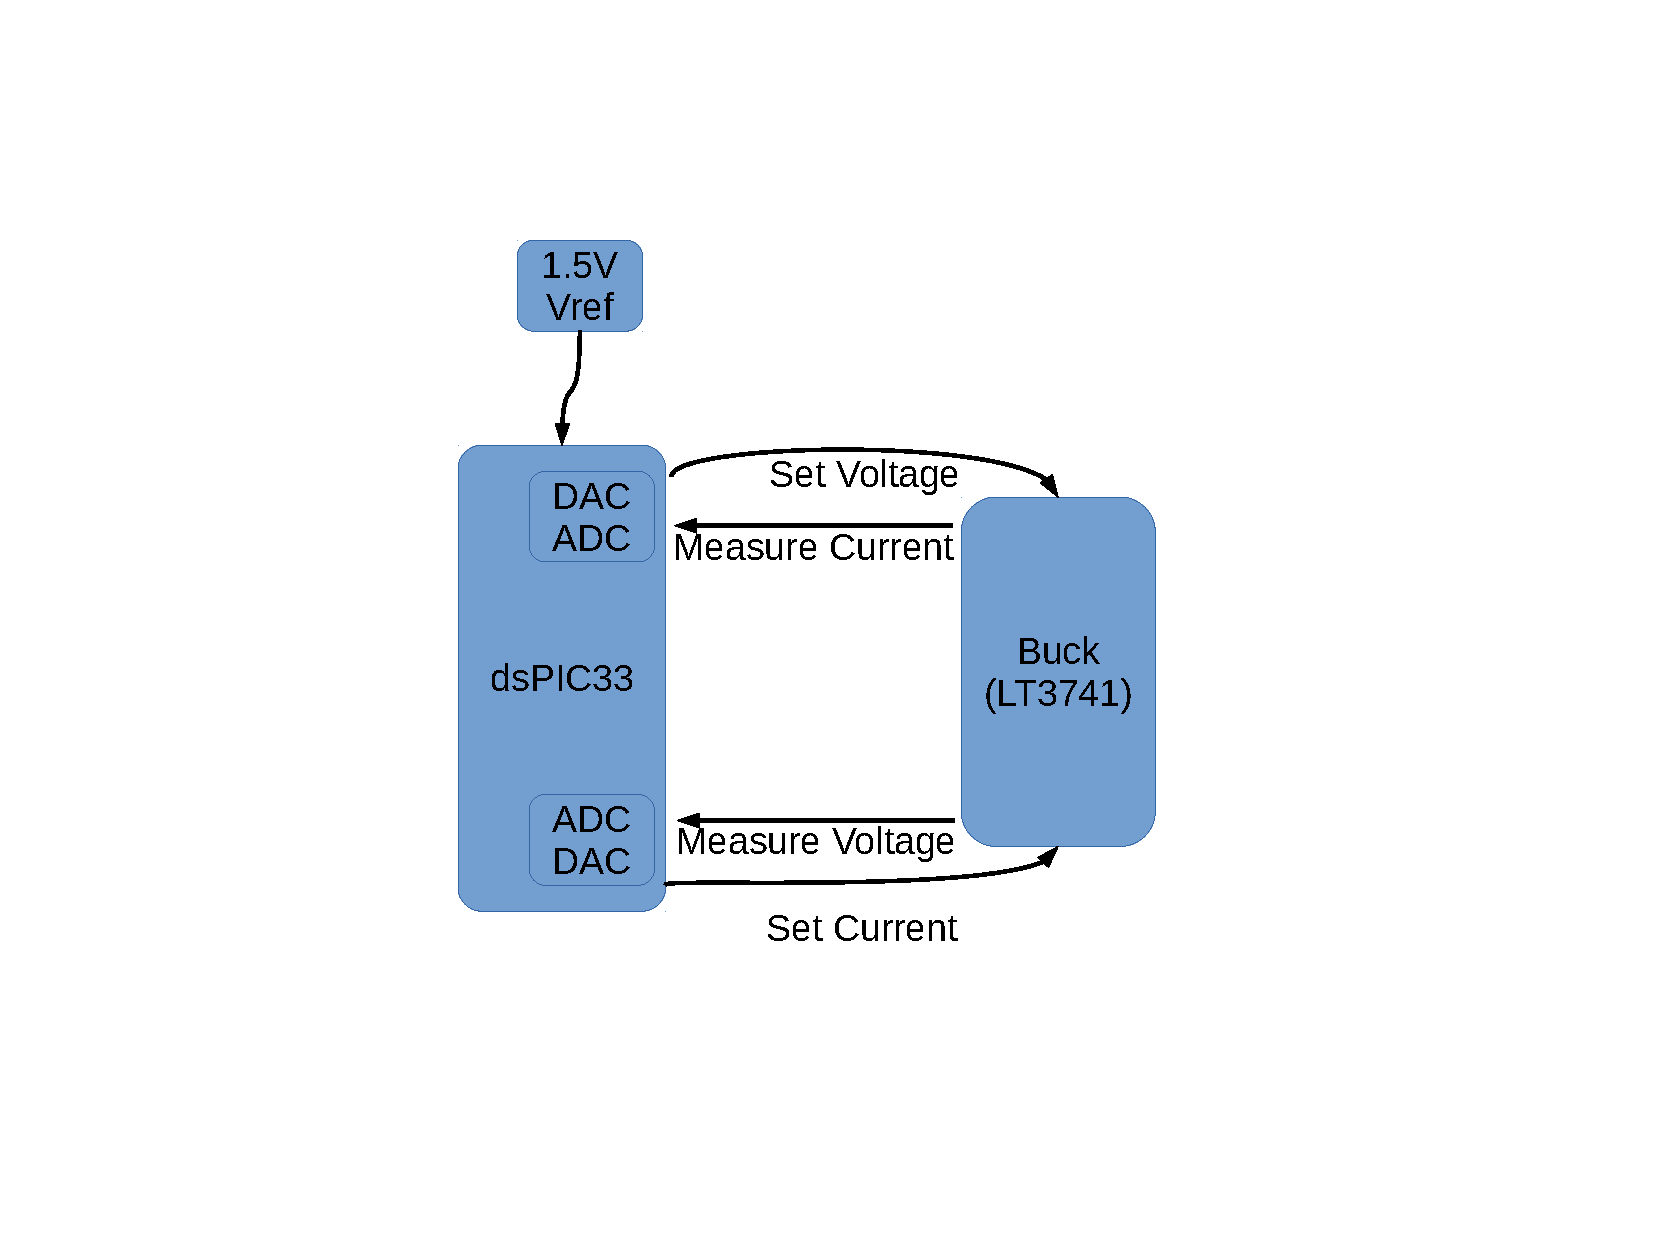
\includegraphics[width=\textwidth,trim=140 140 120 100,clip]{images/block-diag-control.pdf}
    \captionof{figure}{Block diagram of control circuit}
    \label{fig:controlcircuit:schcematic}
\end{minipage}
\begin{minipage}{0.5\textwidth}
    \center
    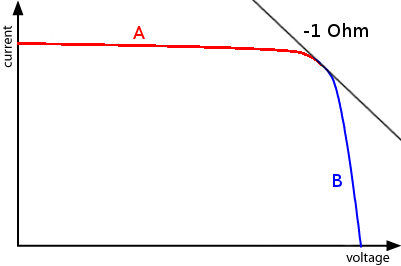
\includegraphics[width=\textwidth]{images/vi-curve.png}
    \captionof{figure}{I-V-Curve with \SI{-45}{\degree} slope indicated}
    \label{fig:controlcircuit:vicurve}
\end{minipage}
